%%%%%%%%%%%%%%%%%%% vorlage.tex %%%%%%%%%%%%%%%%%%%%%%%%%%%%%
%
% LaTeX-Vorlage zur Erstellung von Projekt-Dokumentationen
% im Fachbereich Informatik der Hochschule Trier
%
% Basis: Vorlage svmono des Springer Verlags
%
%%%%%%%%%%%%%%%%%%%%%%%%%%%%%%%%%%%%%%%%%%%%%%%%%%%%%%%%%%%%%

\documentclass[envcountsame,envcountchap, deutsch]{i-studis}

\usepackage{makeidx}         	% Index
\usepackage{multicol}        	% Zweispaltiger Index
%\usepackage[bottom]{footmisc}	% Erzeugung von Fu�noten

%%-----------------------------------------------------
%\newif\ifpdf
%\ifx\pdfoutput\undefined
%\pdffalse
%\else
%\pdfoutput=1
%\pdftrue
%\fi
%%--------------------------------------------------------
%\ifpdf
\usepackage[pdftex]{graphicx}
\usepackage[pdftex,plainpages=false]{hyperref}
%\else
%\usepackage{graphicx}
%\usepackage[plainpages=false]{hyperref}
%\fi

%%-----------------------------------------------------
\usepackage{color}				% Farbverwaltung
%\usepackage{ngerman} 			% Neue deutsche Rechtsschreibung
\usepackage[english, ngerman]{babel}
\usepackage[latin1]{inputenc} 	% Erm�glicht Umlaute-Darstellung
%\usepackage[utf8]{inputenc}  	% Erm�glicht Umlaute-Darstellung unter Linux (je nach verwendetem Format)

%-----------------------------------------------------
\usepackage{listings} 			% Code-Darstellung
\lstset
{
	basicstyle=\scriptsize, 	% print whole listing small
	keywordstyle=\color{blue}\bfseries,
								% underlined bold black keywords
	identifierstyle=, 			% nothing happens
	commentstyle=\color{red}, 	% white comments
	stringstyle=\ttfamily, 		% typewriter type for strings
	showstringspaces=false, 	% no special string spaces
	framexleftmargin=7mm, 
	tabsize=3,
	showtabs=false,
	frame=single, 
	rulesepcolor=\color{blue},
	numbers=left,
	linewidth=146mm,
	xleftmargin=8mm
}
\usepackage{textcomp} 			% Celsius-Darstellung
\usepackage{amssymb,amsfonts,amstext,amsmath}	% Mathematische Symbole
\usepackage[german, ruled, vlined]{algorithm2e}
\usepackage[a4paper]{geometry} % Andere Formatierung
\usepackage{bibgerm}
\usepackage{array}
\hyphenation{Ele-men-tar-ob-jek-te  ab-ge-tas-tet Aus-wer-tung House-holder-Matrix Le-ast-Squa-res-Al-go-ri-th-men} 		% Weitere Silbentrennung bei Bedarf angeben
\setlength{\textheight}{1.1\textheight}
\pagestyle{myheadings} 			% Erzeugt selbstdefinierte Kopfzeile
\makeindex 						% Index-Erstellung


%--------------------------------------------------------------------------
\begin{document}
%------------------------- Titelblatt -------------------------------------
\title{Entwicklung eines rundenbasierten Strategiespiels}
\subtitle{Dokumentation}
%---- Die Art der Dokumentation kann hier ausgew�hlt werden---------------
%\project{Bachelor-Projektarbeit}
\project{Interdisziplin"ares Teamprojekt}
%\project{Master-Projektstudium}
%\project{Master-Abschlussarbeit}
%\project{Seminar zur Vorlesung ...}
%\project{Hausarbeit zur Vorlesung ...}
%--------------------------------------------------------------------------
\supervisor{Prof. Dr. Linda Breitlauch, Prof. Dr. Christof Rezk-Salama} 		% Betreuer der Arbeit
\author{NAMEN PLACEHOLDER} 							% Autor der Arbeit
\address{Trier,} 							% Im Zusammenhang mit dem Datum wird hinter dem Ort ein Komma angegeben
\submitdate{DATUM PLACEHOLDER} 				% Abgabedatum
%\begingroup
%  \renewcommand{\thepage}{title}
%  \mytitlepage
%  \newpage
%\endgroup
\begingroup
  \renewcommand{\thepage}{Titel}
  \mytitlepage
  \newpage
\endgroup
%--------------------------------------------------------------------------
\frontmatter 
%--------------------------------------------------------------------------
\tableofcontents 						% Inhaltsverzeichnis
%--------------------------------------------------------------------------
\mainmatter                        		% Hauptteil (ab hier arab. Seitenzahlen)
%--------------------------------------------------------------------------
% Die Kapitel werden in separaten .tex-Dateien abgelegt und hier eingebunden.
\chapter{Einleitung}

\chapter{Konzeptionierung}


\chapter{Squad Builder}

Der Squad Builder erm"oglicht es beiden Spielern ihre Teams zusammenzustellen. Die Spieler w"ahlen abwechselnd ihre Figuren, bis die vorgegebene Teamgr"o"se erreicht wurde. 

Die linke H"alfte des Bildschirms zeigt die Teamzusammenstellung von Spieler 1. Er kann f"ur jede Einheit einzeln Prim"arwaffe, Sekund"arwaffe und 2 Utility Items w"ahhlen. Die Auswahl erfolgt "uber eigens programmierte Dropdown-Men"us, die sich dynamisch aus den vorgegebenen Enumeratoren und Icon-Listen generieren. Das Best"atigen der Zusammenstellung erfolgt "uber den Bestell-Button unterhalb der linken Anzeigenleiste.   
Die ausgew"ahlten Einheiten werden in der linken Anzeigenleiste durch die ihnen zugeteilte Ausr"ustungsgegenst"ande dargestellt.  

Die rechten drei Buttons erm"oglichen es Spieler 2 seine Figuren aus vorgegebenen Archetypen auszuw"ahlen. Die gew"ahlten Einheiten werden in der rechten Anzeigenleiste durch ihre jeweiligen Icons dargestellt. 


\chapter{Levelaufbau}
Das Level wird durch ein Skript (BattlefieldCreator) aufgrund der Plane generiert. Je gr"o"ser der Localscale der Plane, desto gr"o"ser wird
das Level. Auf einer Skalierung von 1/1/1 entsteht ein 10 * 10 Grid aus Quads(Zellen). Bei Skalierungen im Komma Bereich werden dem entsprechen viele Zellen erstellt. Zum Beispiel bei x = 1,6 und z = 1,7 entsteht ein 16 * 17 Feld.

\begin{lstlisting}[breaklines = true]
 //Initialisiert alle Zellen
 for (float z = 0; z > -(sizeZint); z--) {
	 for (float x = 0; x < (sizeXint); x++) {
		 GameObject zelle = GameObject.CreatePrimitive(PrimitiveType.Quad);
		 zelle.transform.Rotate(new Vector3(90, 0, 0));
		 zelle.AddComponent<Cell>();
		 zelle.tag = "Cell";
		 zelle.name = x + "|" + -z;
		 zelle.transform.position = new Vector3((x + 0.5f), 0.001f, (z - 0.5f));
\end{lstlisting}

Die Objekte werden durch das Skript ObjectSetter beim Spielstart auf dem Grid platziert. Sollte ein Objekt gr"o"ser als eine Zelle sein so wird dies in der ObjectComponent durch X und Z wert angegeben. Ebenso wird dort vermerkt ob das Objekt Deckung bietet und die Zelle besetzt.


\begin{figure}
	\centering
	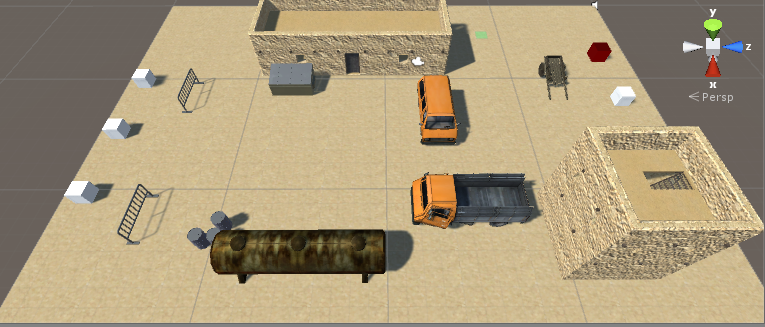
\includegraphics[height=6cm]{images/FinalLevel.png}
	\caption{Das finale Level mit Spieleraufstellung}
	\label{fig:FinalLevel}
\end{figure}
\chapter{Manager Objekt}

Um die verschiedenen Systeme, die f"ur den korrekten Ablauf der Spielz"uge und allgemein spielregeltechnischen Abl"aufe zu handeln, wurde ein Spielobjekt, das als Manager bezeichnet wird, erstellt. Im folgenden Kapitel wird auf die einzelnen Skripte die an diesem Manager Objekt h"angen genauer eingegangen. 

\section{Manager System}

Das Manager System ist für den korrekten Ablauf der einzelnen Züge zuständig. Es z"ahlt die Runden hoch, stellt sicher, dass nur das die Eingabe des Spielers, der aktuell an der Reihe ist, abgehandelt wird, merkt sich die aktuell ausgew"ahlte Spielfigur, damit das User-Interface korrekt dargestellt wird, f"ugt jedem Spieler seine Spielfiguren zu und setzt die Spielfiguren zu Beginn der Sitzung an zuvor festgelegte Positionen.

\section{Shooting System}

Das ShootingSystem beschreibt das Schussverhalten der verschiedenen Waffen im Spiel. Dabei werden hier verschiedene Boni und Mali auf die Angriffskraft der Waffe verteilt, um so situationsabh"angig agieren zu k"onnen. Zum Beispiel wird auch die Distanz zum Gegner in Betracht gezogen . Die Ver"anderung des Angriffs wird wie folgt unterteilt. \newline
Einen Bonus erh"alt man, wenn sich das Ziel nahe dem Angreifer befindet oder das Ziel sich nicht hinter einer Deckung aufh"alt. \newline
Einen Malus erh"alt man, wenn sich das Ziel weit weg vom Angreifer, hinter einer hohen Deckung oder im Nebel einer Rauchgranate befindet.\newline

Hinzu kommt noch die Frage ob ein Spieler "uberhaupt die M"oglichkeit besitzt zu schie"sen, dies kann durch mangelnde Ressourcen wie Munition der Fall sein.
Desweiteren wird eine Wahrscheinlichkeit berechnet, die zuf"allig bestimmt, ob ein Spieler seinen Gegner trifft, diese steigt jedoch je besser sich der Angreifer mit den oben erw"ahnten Boni aufgestellt hat.


\section{Inventory System}

Das Inventory System wird aufgerufen sobald ein Spieler eine der folgenden Aktionen ausf"uhrt um die Anzahl der im Inventar der Spielfigur enthaltenen Gegenst"ande zu verringern:\newline


\begin{itemize}
	\item Nachladen der Prim"arwaffe
	\item Einsatz von Handgranaten
	\item Einsatz von Tr"anengas
	\item Einsatz von Rauchgranaten
	\item Einsatz von Molotovcocktails
\end{itemize}





\section{Player Assistance System}



\section{Ability System}



\section{Health System}

Die Schadensberechnung sowie auch Heilung erfolgt durch das HealthSystem. Hierf"ur wird für die Schadensberechnung beispielsweise die Angriffskraft der Waffe betrachtet. Beim Einsatz eines Medipacks wird einfach ein definierter Wert an Lebenspunkten wieder hergestellt.
Der eigentliche Vorgang wird dabei unterteilt in Berechnung des Schadens- bzw. Heilwertes und das entsprechende ver"andern der Werte, dies sorgt für weitere "Ubersicht und l"asst sich wie folgt verbildlichen:

\begin{lstlisting}[breaklines = true]
public void doDamage(AttributeComponent attackingPlayerAttr, PlayerComponent attackingPlayerComp, AttributeComponent damageTakingPlayerAtrr, int damageFlag)
{
switch(damageFlag)
{
case SHOOT:
int damage = generateShootDamage(attackingPlayerAttr, damageTakingPlayerAtrr);
inflictShootDamage(attackingPlayerAttr, attackingPlayerComp, damageTakingPlayerAtrr, damage);                    
break;

default:

break;
}
}
\end{lstlisting}


\chapter{Spieler}

Das Spieler Objekt enth"alt als Kindobjekte seine Spielfiguren. Als Skripte h"angen ihm eine Player Component, sowie eine Input Component an. 
\section{Player Component}
\begin{lstlisting}[breaklines=true]
GameObject[] figurines = new GameObject[3]; //Alle Figuren ueber die ein Spieler verfuegt
public int actionPoints = 0; //Anzahl an verfuegbaren Aktionspunkten
int maxAP; //Maxcap für AP
\end{lstlisting}
Das Skript speichert die maximale Anzahl an Aktionspunkten, die f"ur die verschiedenen Fraktionen variieren, f"ullt nach dem Ende der Runde die Aktionspunkte beider Fraktionen auf und stellt sicher, dass dabei die Zahl der erhaltenen Aktionspunkte nicht die Grenze "uberschreiten. 

\begin{figure}
	\centering
	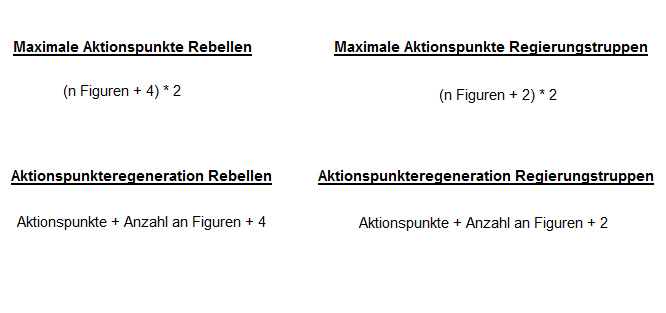
\includegraphics[height=5cm]{images/Aktionspunkte.png}
	\caption{Berechnung der Aktionspunkte}
	\label{fig:Aktionspunkte}
\end{figure}

\section{Input System}
Jedes Spielerobjekt, welches die verschiedenen Spielfiguren besitzt, besitzt jeweils ein Input System.
Dieses Inputsystem ist f"ur das Starten von Aktionen, sowie die Auswahl von Zielen oder Figuren zust"andig. Mit Hilfe von Raycasts in die Szene hinein, wird ermittelt, welches Objekt oder Zelle getroffen wird. 

Das Input System wird auch durch das UI System benutzt. Wenn Buttons f"ur Aktionen gedr"uckt werden, wird im Input System die entsprechende Aktion ausgew"ahlt, die als n"achstes ausgef"uhrt werden soll. Diese Aktionen werden dann an die entsprechenden Systeme (Movement- , Ability- oder Shooting Sytem) weitergegeben, wo die Logik ausgef"uhrt wird.
\chapter{Spielfiguren}

\section{Bewegung}
Bei unseren Spielfiguren um kleine Plastiksoldaten handelt, die sich in einem kindlich dargestelltem Nah-Ostkonflikt befinden. Die Bewegung der Einheiten wird daher "uber eine Parabelkurve angedeutet, an der sich die Figur beim laufen entlang bewegt. Somit wird der Eindruck erzeugt, die Figur werde wie von einer unsichtbaren Hand in einem Brettspiel "uber das Feld bewegt.

\section{Attribute Component}
Die Attribute Component dient dazu, die spieletechnischen Werte der Figur abzuspeichern. Sollte es sich um eine Figur aus der Fraktion "Regierungstruppen" sein wird die Attribute Component mit den passenden Werten initialisiert, die f"ur die ausgew"ahlte Klasse vordefiniert wurden. Handelt es sich um eine Figur aus der Fraktion "Rebellen" wird diese mit den Ausr"ustungsgegenst"anden best"ueckt. 


\section{Inventory Component}
Jeder einzelnen Spielfigur wird eine Inventory Component angehangen. In dieser wird das gesamte Inventar der jeweiligen Figur gespeichert. Das Inventory System k"ummert sich dabei um die Berechnungen und Aktualisierung der Inventory Komponenten.\newline
Es folgt ein Auszug der verschiedenen Variablen:\newline

\begin{lstlisting}[breaklines = true]
//Inventar (primaerwaffe, sekundaerwaffe, equipment1, equipment2) siehe Enums.cs    
public Enums.PrimaryWeapons primaryWeaponType;
public Enums.SecondaryWeapons secondaryWeaponType;
public Enums.Equipment utility1;
public Enums.Equipment utility2;

public WeaponComponent primary; //Primaerwaffe
public WeaponComponent secondary; //Sekundaerwaffe
public bool isPrimary; //Ist Primaerwaffe ausgewaehlt? 
public int amountSmokes; //Anzahl Rauchgranaten
public int amountTeargas; //Anzahl Teargas
public int amountGrenades; //Anzahl Granaten
public int amountMolotovs; //Anzahl Molotovs
public int amountMediKits; //Anzahl Medikits
public int amountMagazines; //Anzahl Magazine//Anzahl Magazine
\end{lstlisting}


\chapter{Pathfinding}

\chapter{Kamera}

Die Kamera ist eine beweglich Orbitkamera mit Zoom und Rotation die sich nur innerhalb des Levels bewegen kann. Realisiert wird dies durch einen konstanten Focus auf ein bewegliches, unsichtbares Objekt. Die Kamera l"asst sich "uber das Feld bewegen in dem die Maus an den jeweilige Rand bewegt wird der in die gew"unschte Richtung f"uhrt.

Die folgende Funktion pr"uft ob die Kamera im Feld ist:

\begin{lstlisting}[brealines = true]
	public bool inBattlefield()
	{
		bool inField = true;
		if (target.transform.position.x < 0) {
			inField = false;
			target.transform.position = new Vector3(0, target.transform.position.y, target.transform.position.z);
		}
		if (target.transform.position.z > 0) {
			inField = false;
			target.transform.position = new Vector3(target.transform.position.x, target.transform.position.y, 0);
		}
		if (target.transform.position.x > (plane.transform.position.x * 2)) {
			inField = false;
			target.transform.position = new Vector3((plane.transform.position.x * 2), target.transform.position.y, target.transform.position.z);
		}
		if (target.transform.position.z < (plane.transform.position.z * 2)) {
			inField = false;
			target.transform.position = new Vector3(target.transform.position.x, target.transform.position.y, (plane.transform.position.z * 2));
		}
	return inField;
	}
\end{lstlisting}

\chapter{User-Interface}
Das UI besteht aus verschiedenen Komponenten.

\section{Action-Points Leiste}
Die Aktionspunkte Leiste am oberen Bildrand zeigt für beide Spieler die maximalen sowie die aktuell verfügbaren Aktionspunkte an

\section{Dynamische Ability-Icons}
Wenn ein Spieler eine Einheit auswählt, so werden am unteren Bildrand die erforderlichen Aktionsbuttons angezeigt. Es werden nur die Buttons dargestellt, deren Aktionen von der ausgewählten Figur durchgeführt werden können. 

\section{HP Leisten}
Durch drücken der Leertaste können für alle Figuren Segmentanzeigen dargestellt werden, die die aktuellen Lebenspunkte wiederspiegeln. Jedes Segment steht dabei für 10 Lebenspunkte.
\chapter{3D Modelling}
Sowohl die Charaktere als auch Assets wurden ausschlie"sslich in Blender gemodelt. Hierbei wurde sich stark an reellen Vorgaben, was Kleidung oder einpr"agsame Details betrifft, orientiert. Um den angestrebten Lowpoly-Stil konstant umzusetzen wurden teilweise erst Highpoly-Modelle erstellt um diese in der sogenannten ``retopology`` sp"ater detailarmer zu gestalten.

\begin{figure}
	\centering
	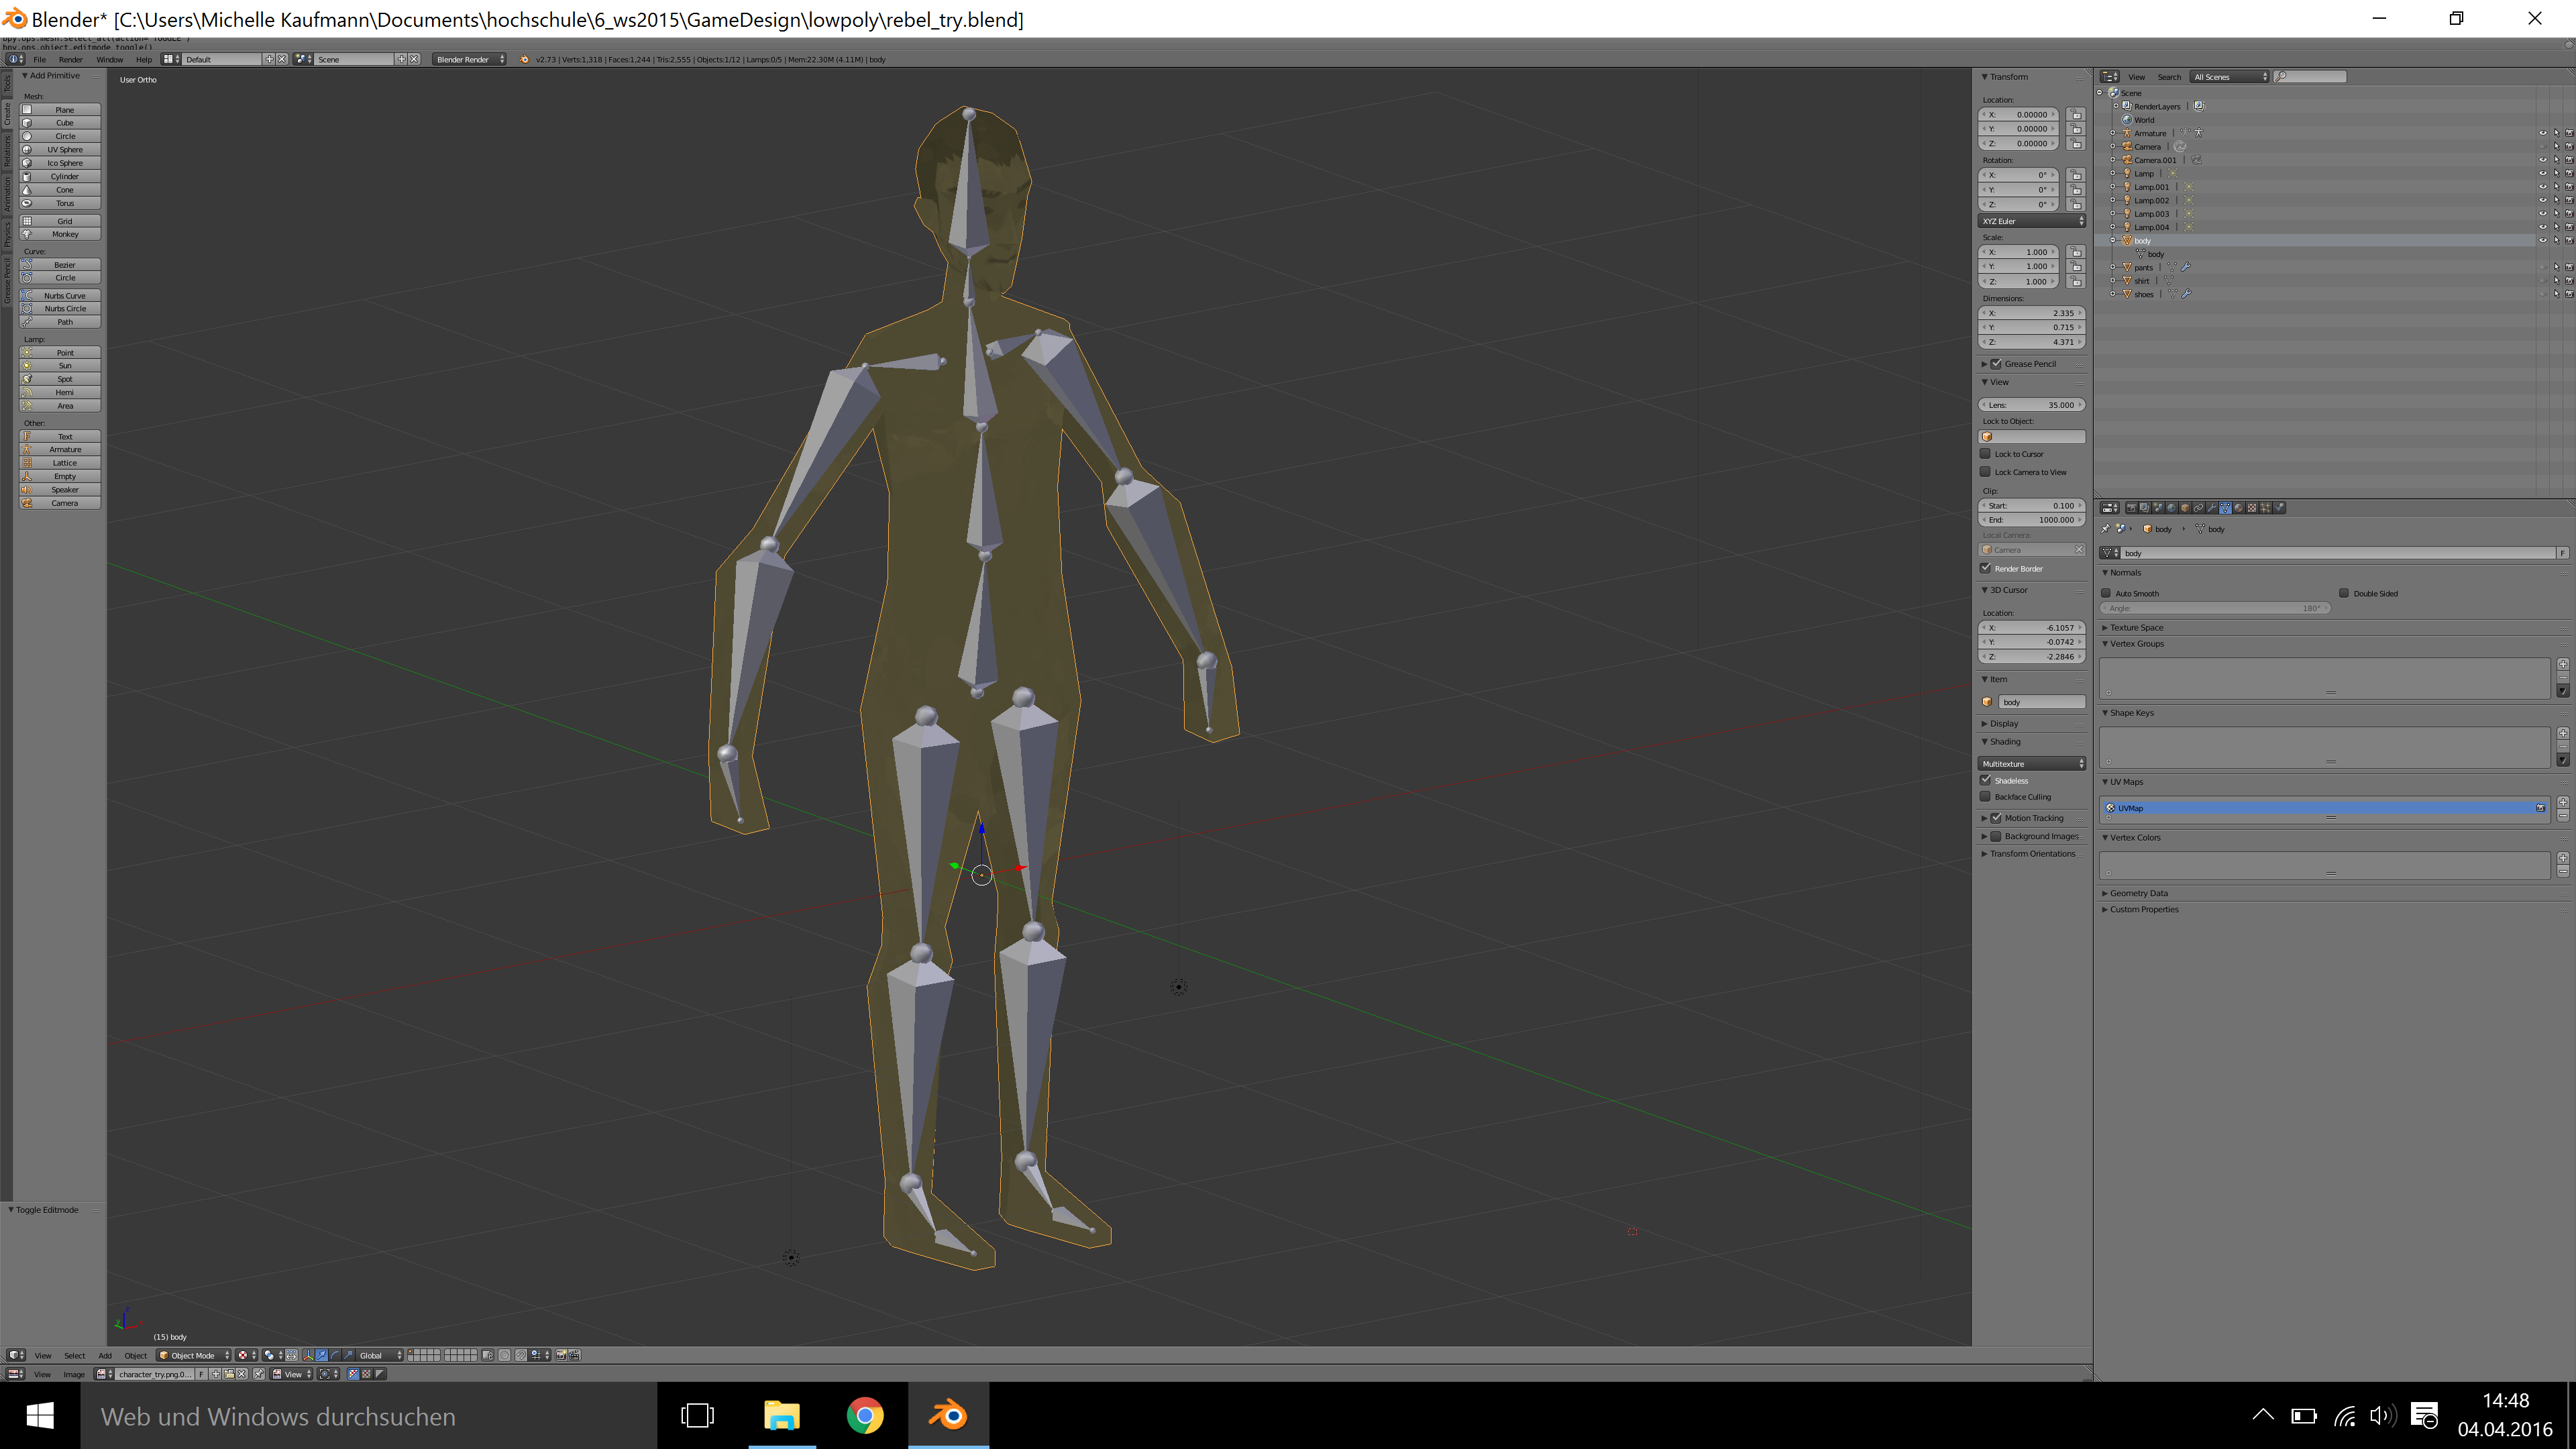
\includegraphics[height=6cm]{images/screenshot3.png}
	\caption{Charaktermodell in Blender}
	\label{fig:charmodell}
\end{figure}

\begin{figure}
	\centering
	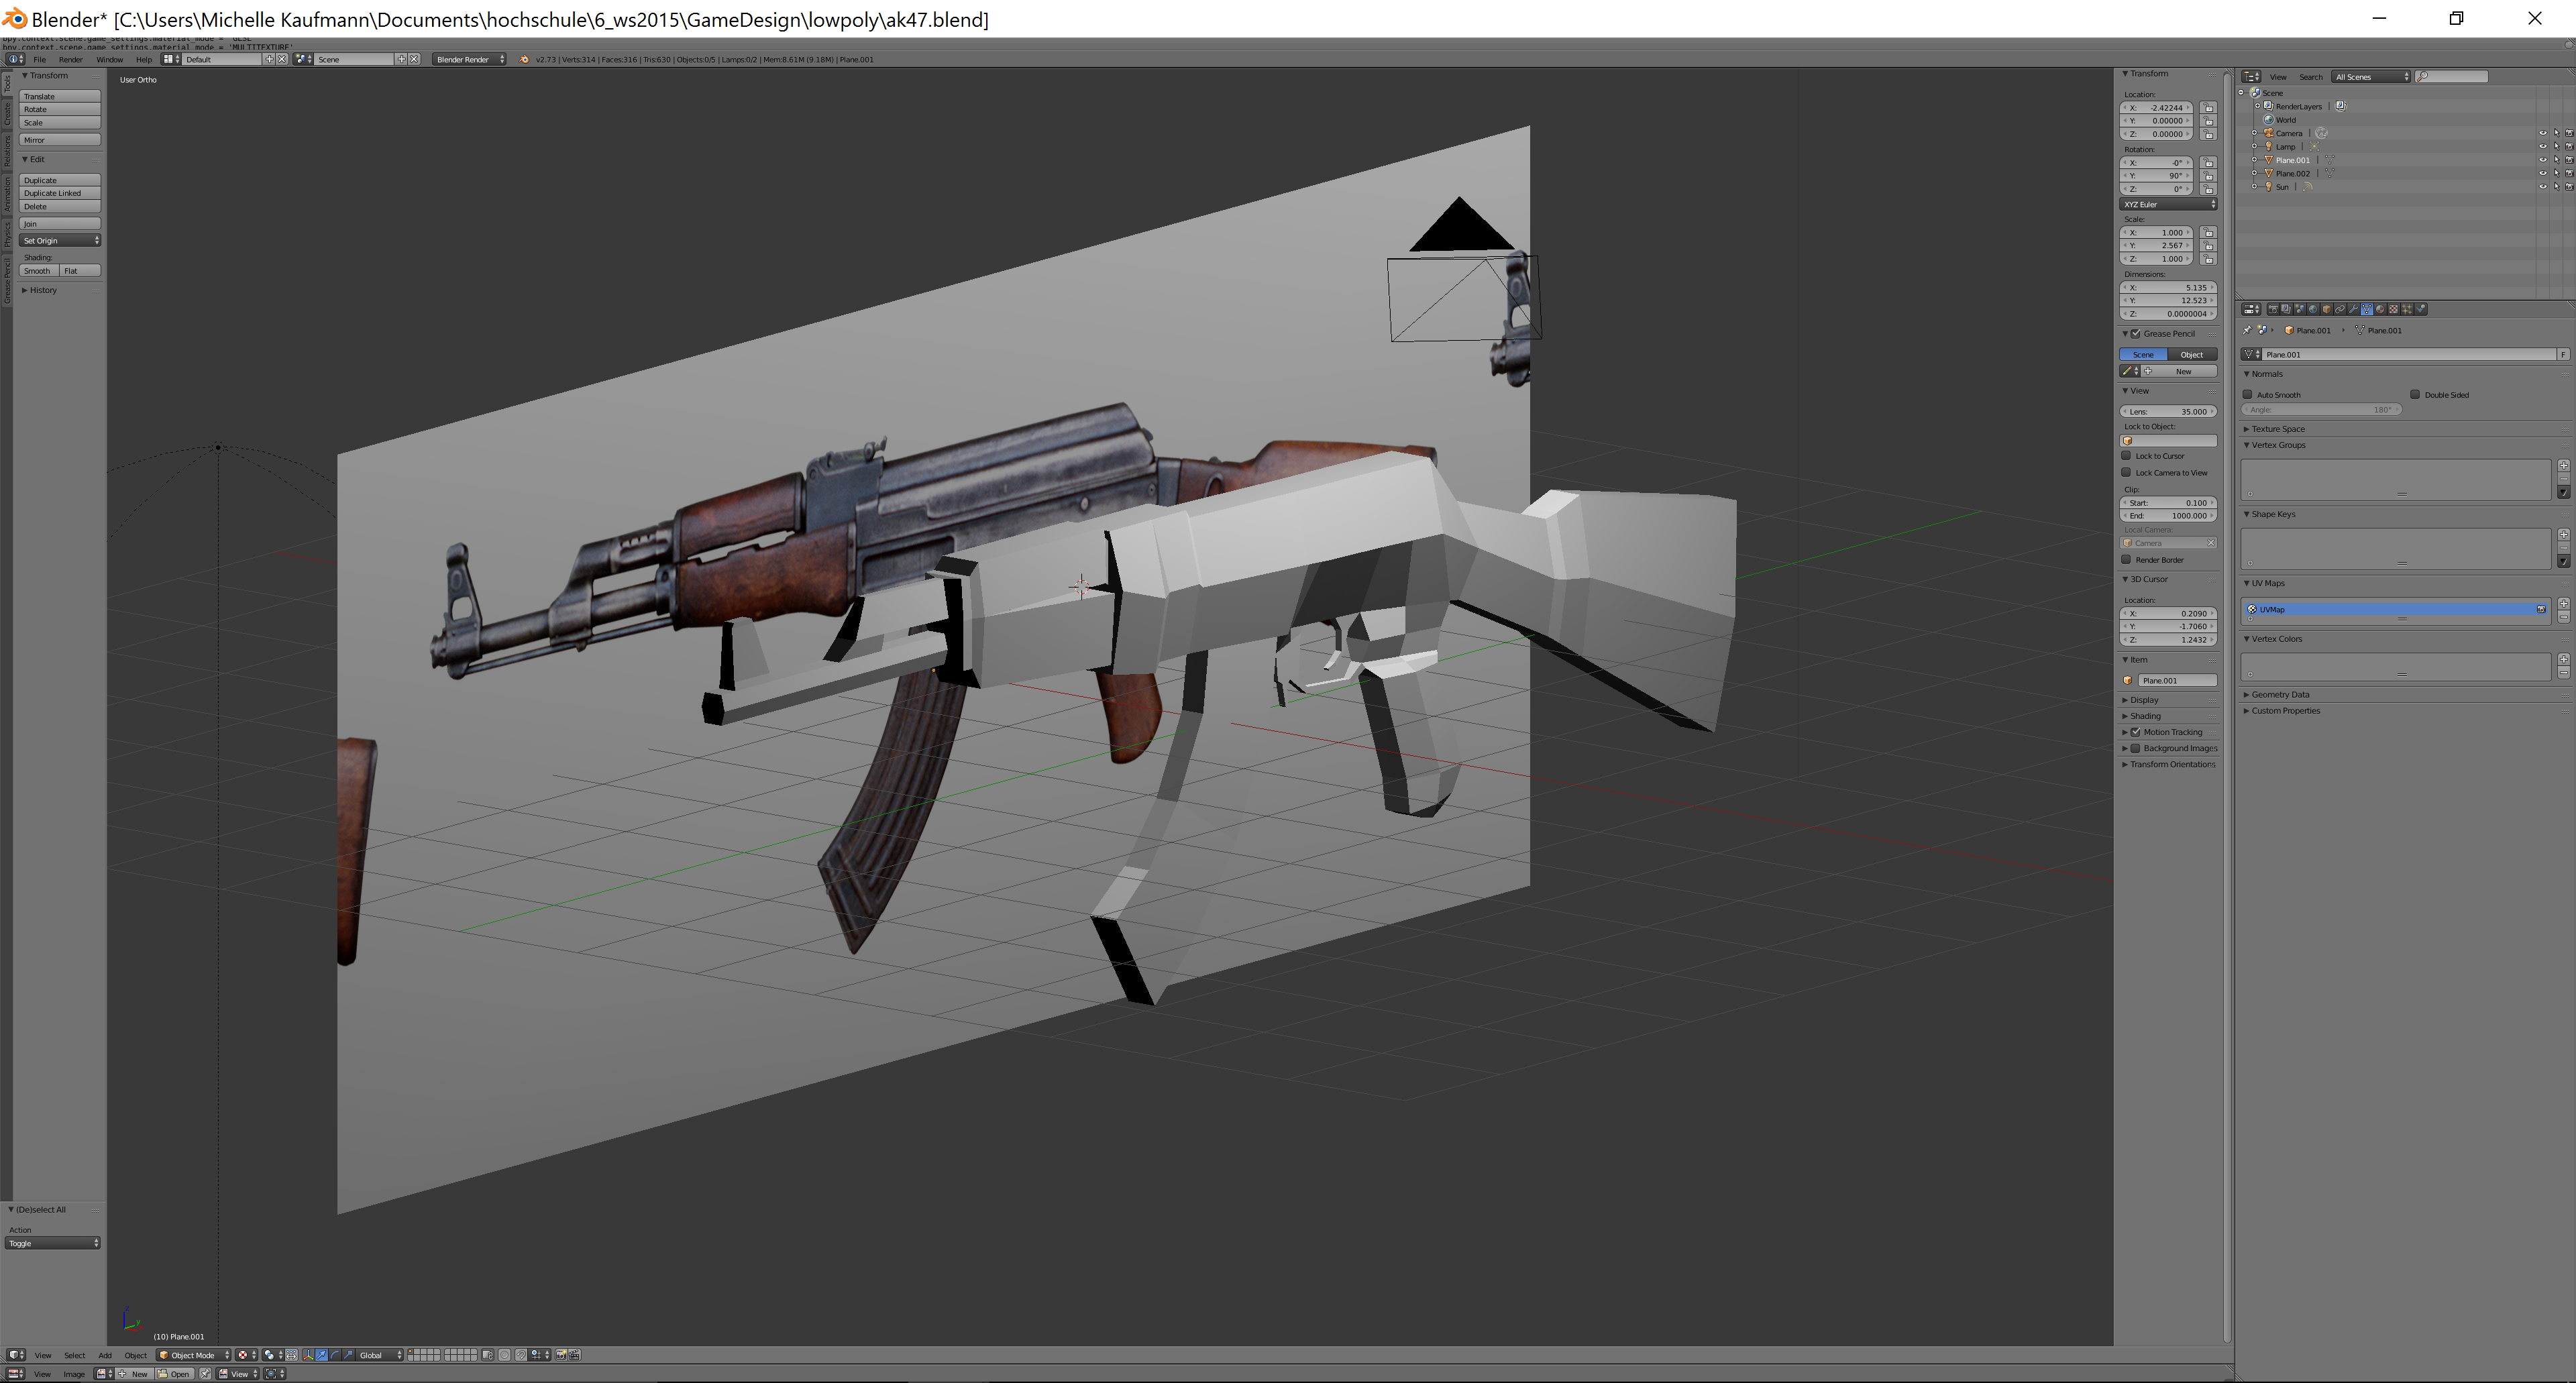
\includegraphics[height=6cm]{images/screenshot2.png}
	\caption{Waffenmodellierung in Blender}
	\label{fig:akmodel}
\end{figure}

\begin{figure}
	\centering
	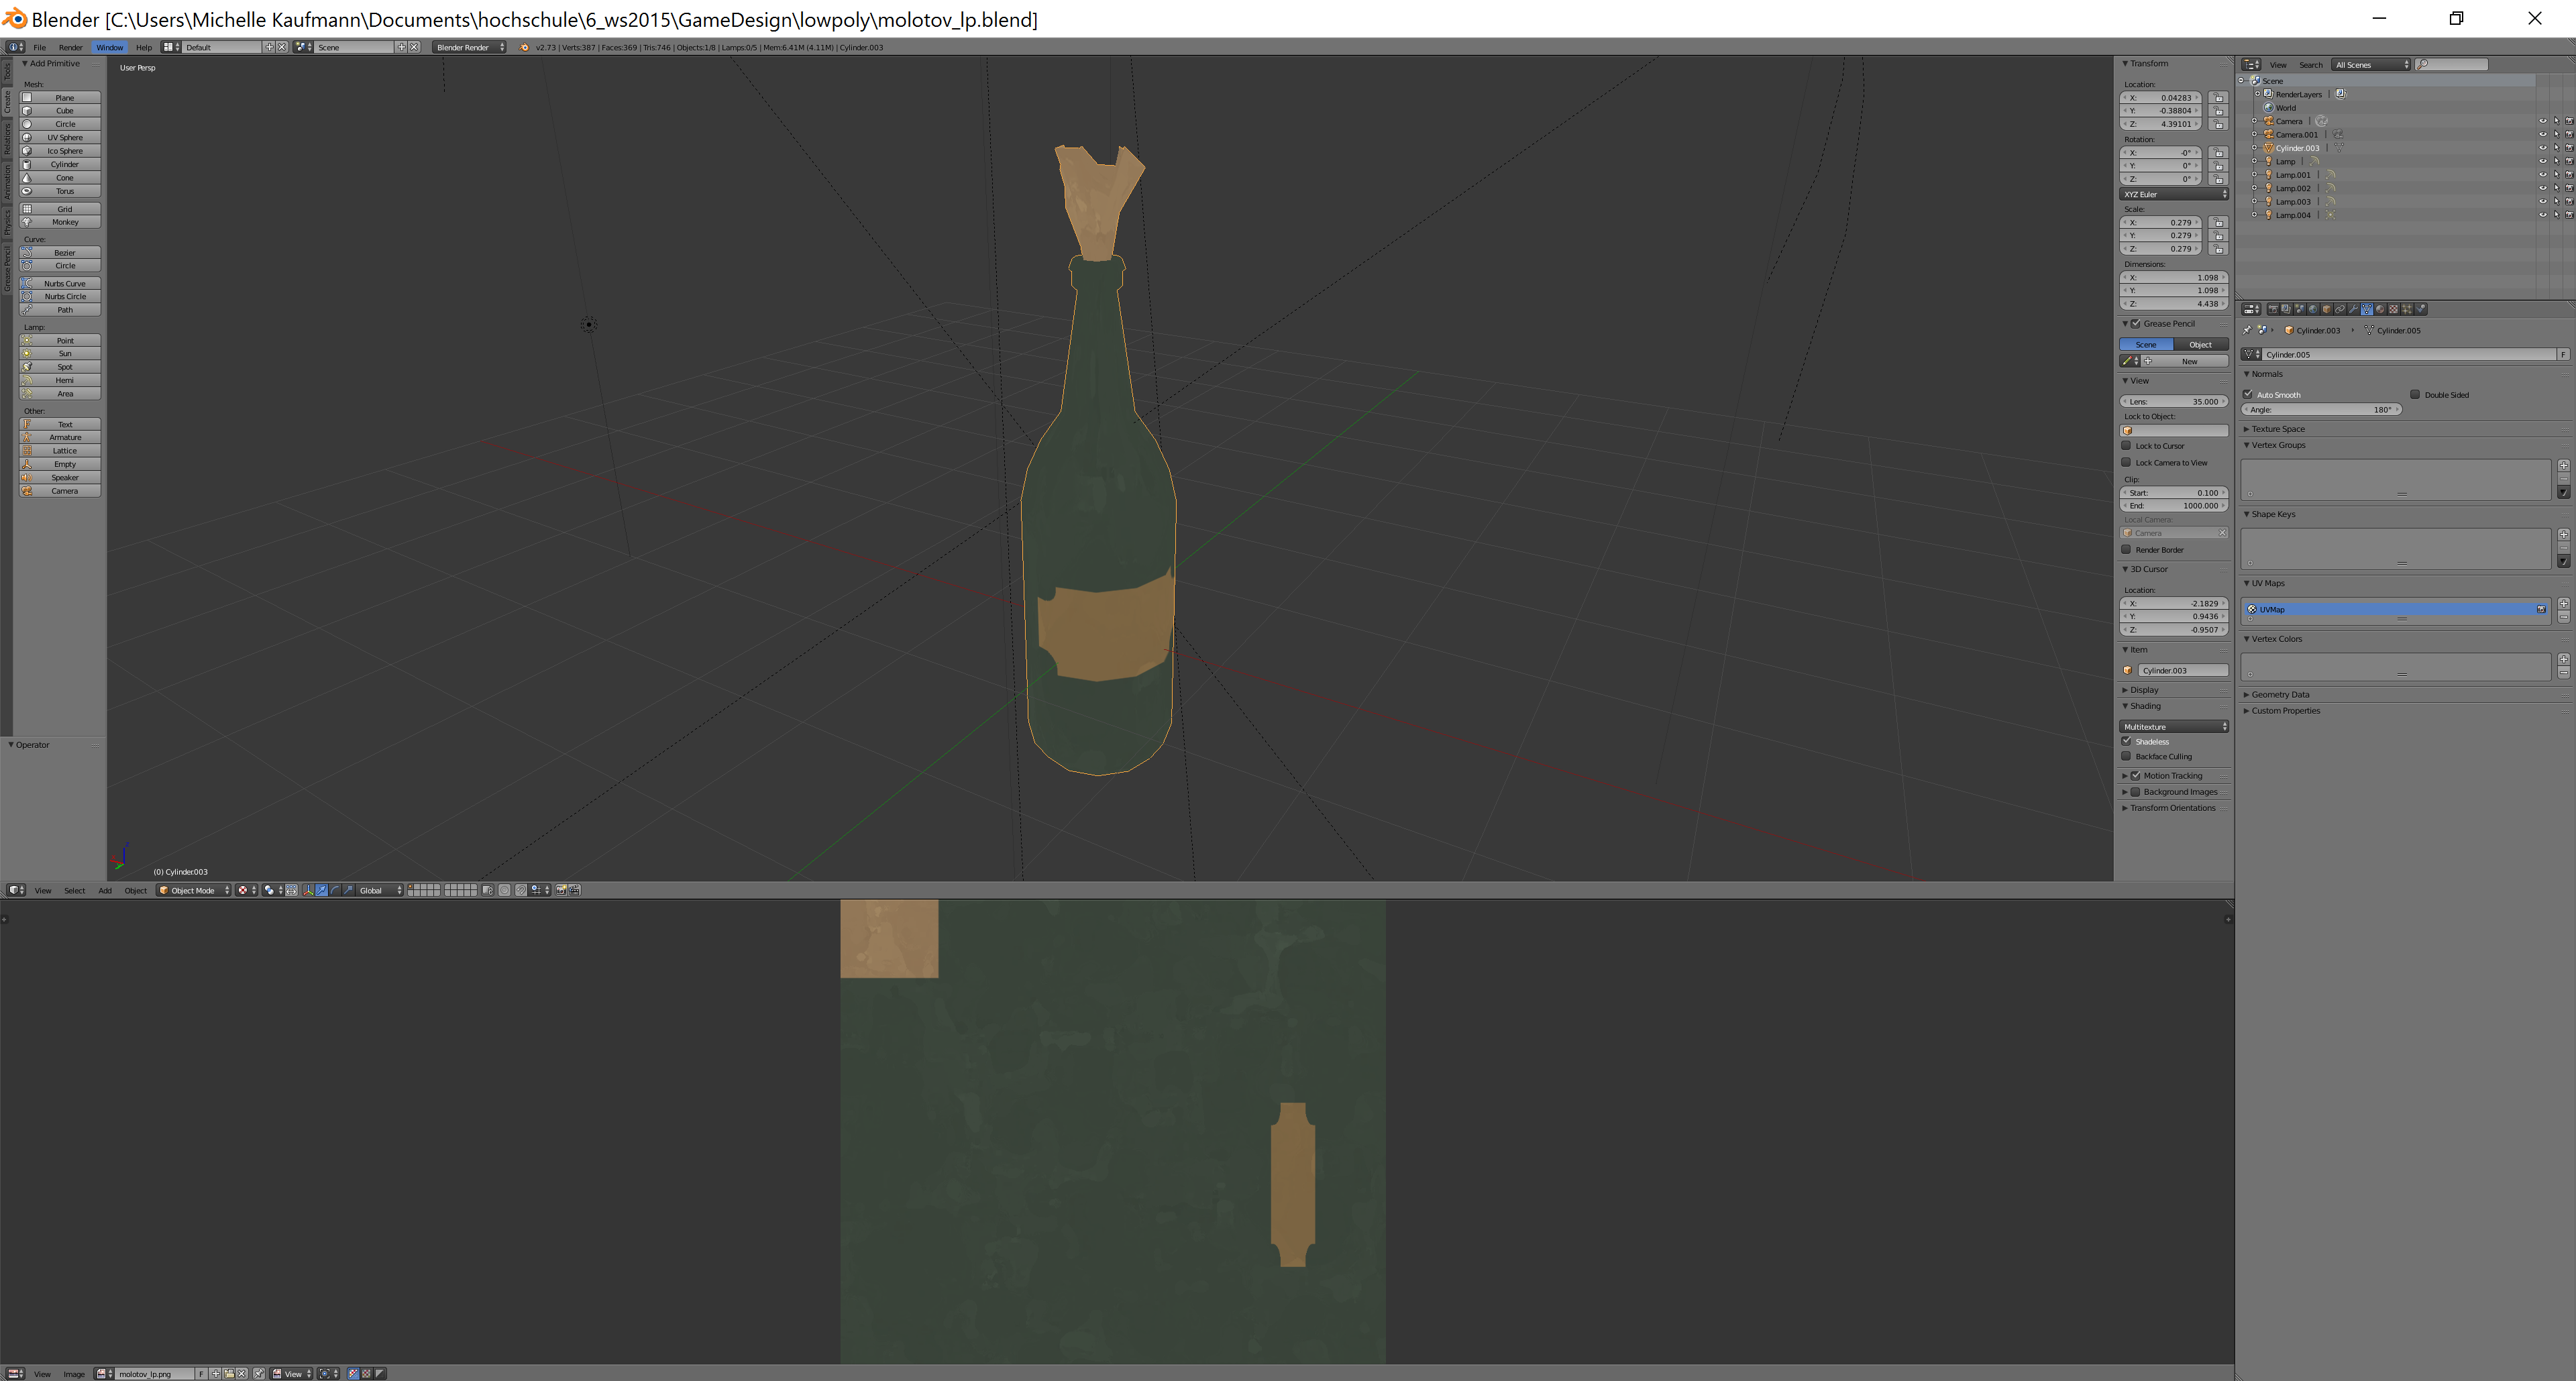
\includegraphics[height=6cm]{images/screenshot4.png}
	\caption{Propmodellierung in Blender}
	\label{fig:molotovmodel}
\end{figure}

\begin{figure}
	\centering
	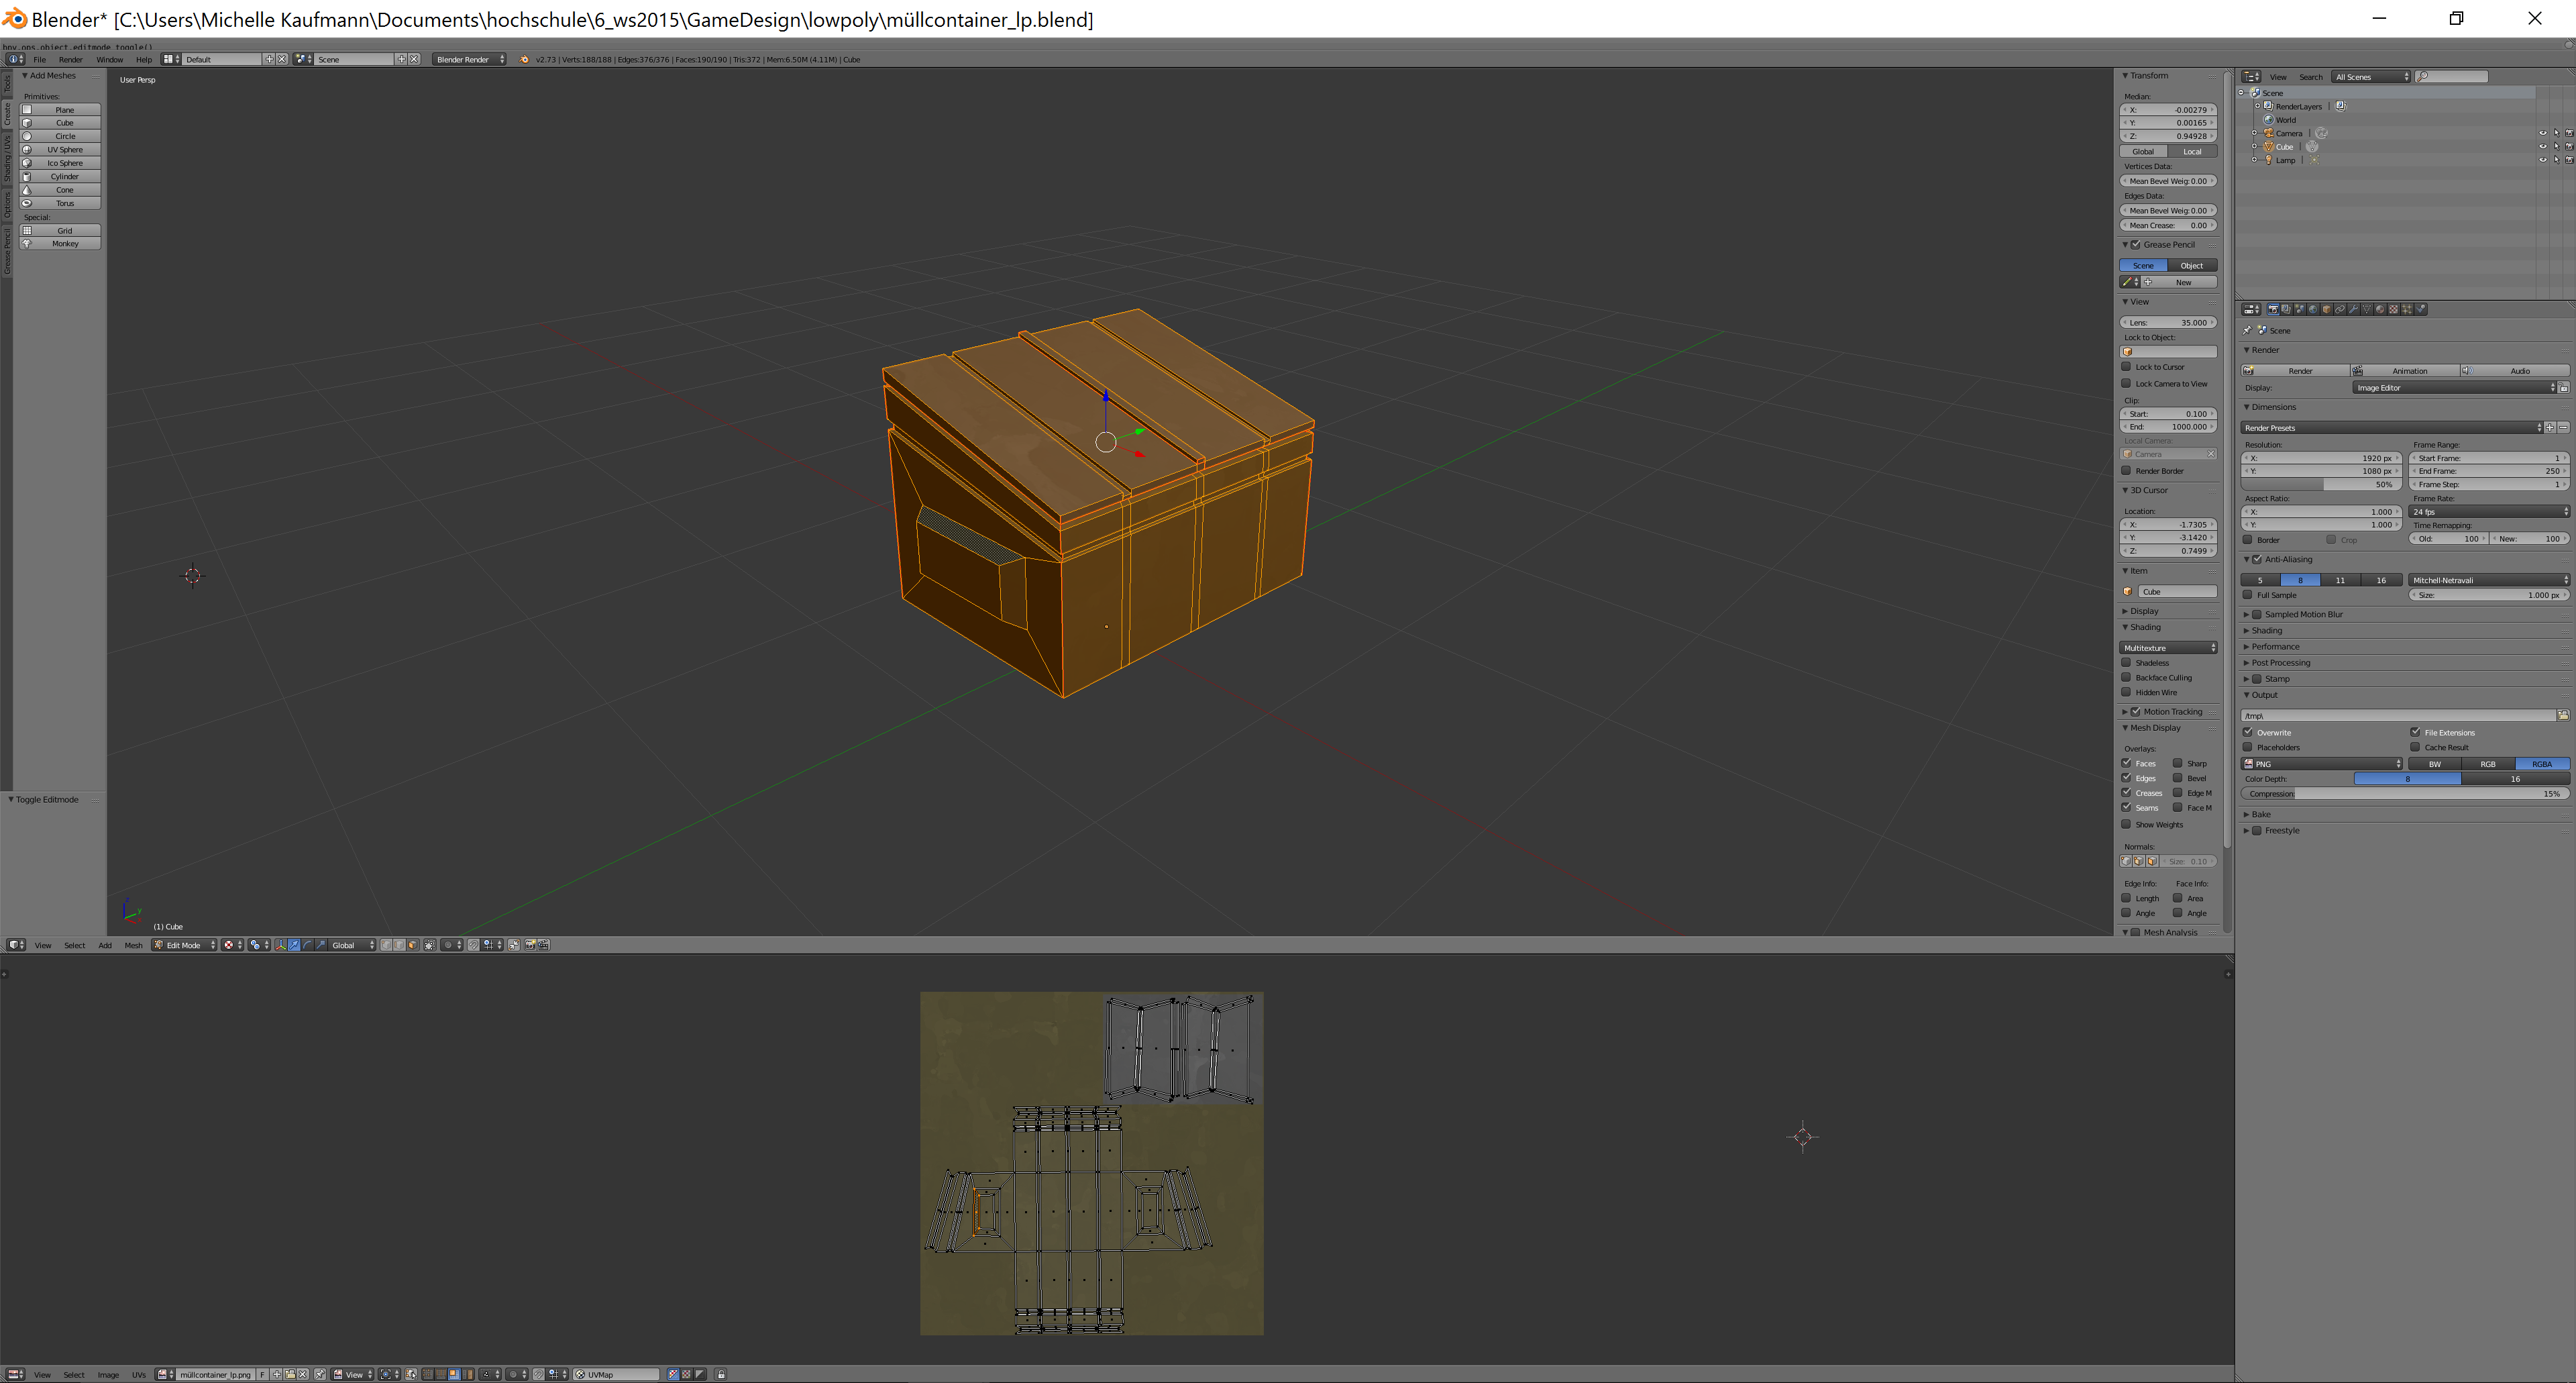
\includegraphics[height=6cm]{images/screenshot1.png}
	\caption{Propmodellierung in Blender}
	\label{fig:containermodel}
\end{figure}
\input{chapters/Animationen}
\input{chapters/Sounds}
\chapter{Effekte}
F"uer die veschiedenen F"ahigkeiten sowie schie"sen wurden Partikeleffekte erstellt.
Dazu wurde das Partikelsystem von Unity genutzt.

\begin{figure}
	\centering
	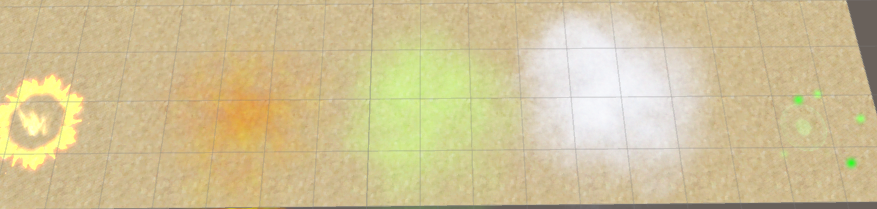
\includegraphics[height=4cm]{images/Partikeleffekte.png}
	\caption{Von Links nach Rechts: Explosion, Feuer, Gas, Rauch, Heileffekt}
	\label{fig:Effekte}
\end{figure}

\chapter{Status quo}

Cursor Feedback welche Aktion ausgewaehlt wird. 
\chapter{Fazit}
Schlussendlich lie"s s

%\input{chapters/TeilnehmerInterviews}
% ...
%--------------------------------------------------------------------------
\backmatter                        		% Anhang
%-------------------------------------------------------------------------
\bibliographystyle{geralpha}			% Literaturverzeichnis
%\bibliography{literatur}     			% BibTeX-File literatur.bib
%--------------------------------------------------------------------------
\printindex 							% Index (optional)
%--------------------------------------------------------------------------
%\begin{appendix}						% Anh�nge sind i.d.R. optional
%   \chapter{Glossar}
			% Glossar   
%\end{appendix}

\end{document}
